\chapter{Methodology} \label{methodology}
In this chapter we will explore the approaches followed to plan, organise, manage and develop the project. We will discuss the methodologies that were adapted and combined to complete the research and development of the project along with why they were implemented. This section aims to give insight to the reader how the project transformed from research to final software while collaborating as a team.

Throughout our four years at GMIT a major emphasis was always placed on the importance of software development methodologies and the importance of choosing the most suitable methodology for a given project. There are numerous  methodologies that have all been extensively explored such as Waterfall, RAD (Rapid Application Development) and Extreme Programming to name a few. For this project we chose the main modern leader also based on the methodologies used by our employers, an approach known as Agile programming.

% ========================== Version Control  ========================== 
\section{Version Control}
\begin{figure}[H]
\begin{minipage}{.5\textwidth}  %listing bloc will have 50% of the line width 
\lstset{linewidth = 4cm, breaklines=true} %set your listing lines widths, and set breaklines to true
In regards to version control with a focus on collaboration we decided to use the online GitHub Source Control Software. GitHub is a development platform allowing users to host and review code while also functioning as a simple yet powerful project management tool. Allowing the team to collaborate and support every aspect of the project management in one place it was an easy decision. 

\end{minipage}
\qquad %space between listing bloc and the figure
\begin{minipage}{0.4\textwidth} %figure will have the remaning 40% of the line width
 
\includegraphics[width=\linewidth]{img/git.jpeg}
\caption{The Agile Cycle}
\end{minipage}
\end{figure}

GitHub enabled us to set up a team organisation that could store both our dissertation and our applied project repository's. We took full advantage of the many features that Github has to offer. The main function of Github allowed us to commit our work to the repositories and merge changes into the existing project. Another effective feature of Github is the project section, which is used to optimize project management. With a built in Kanban board we were able to track our progress while also logging any bugs or issues that arise \textit{(more details on this are given in Section \ref{KanbanSection})}. In respect to Software Development another impressive feature of Github is the ability to create branches. Essentially a branch is a pointer to a unique set of modifications to the original "Master" branch and is given its own branch name. Creating separate branches allows us to work on features and experiment with different functions without having an effect on the main project. When each feature is tested and complete, Github simple allows us to \textit{merge} our new changes back into the main \textit{master} branch.

% ========================== Development approach  ========================== 
\section{Agile development approach}
Agile Software Development is a concept that allows a product be delivered to the customer in incremental releases while also being highly flexible, allowing requirements to change and the scope of the project to increase without major consequences on the design or current task\cite{agile}.

We chose Agile as it stood out and had many benefits to our own project:

\begin{figure}[H]
\begin{minipage}{.5\textwidth}  %listing bloc will have 50% of the line width 
\lstset{linewidth = 4cm, breaklines=true} %set your listing lines widths, and set breaklines to true
\begin{itemize}
\item Develop small, incremental releases
\item Active user involvement
\item Evolving requirements
\item High level requirements
\end{itemize}

\end{minipage}
\qquad %space between listing bloc and the figure
\begin{minipage}{0.4\textwidth} %figure will have the remaning 40% of the line width
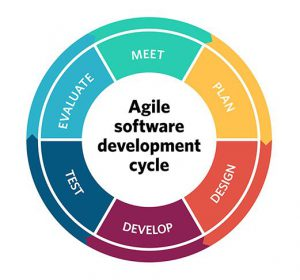
\includegraphics[scale=.4]{img/agile.jpg} %the image must be resized or scaled if needed
\caption{The Agile Cycle}
\end{minipage}
\end{figure}

Firstly as we were exploring all new languages, frameworks and libraries Agile allowed us to easily continuously integrate new features as our knowledge portfolio grew. Another major advantage was that this approach allowed us to have a working model every week rather than releasing the project in one release as would be in the Waterfall methodology. This alone gave us the opportunity to review each weeks progress while also receive continuous feedback from our mentors.

From the outset of the planning phase the main requirements and features of the software were identified. Subsequently we broke these features down into sub tasks which enabled complex tasks to be completed with simplicity. In the following subsections we will explain how using two prominent features of Agile, namely Kanban and Sprints we could track our development and monitor our progress.


% ========================== KanBan  ========================== 
\subsection{KanBan} \label{KanbanSection}
The Kanban Method is a means to design, manage, and improve flow systems for knowledge work. The method also allows organizations to start with their existing workflow and drive evolutionary change. They can do this by visualizing their flow of work, limit work in progress and stop starting and start finishing \cite{kanban}.

The Kanban Method gets its name from the use of kanban - visual signaling mechanisms to control work in progress for intangible work products. In simplicity Kanban is based around a Kanban board featuring Kanban cards (sticky notes). Thus allowing the full team to visualize crucial project information such as what tasks need doing, what tasks are in progress (and by whom) and what tasks are complete. 

\begin{figure}[H]
  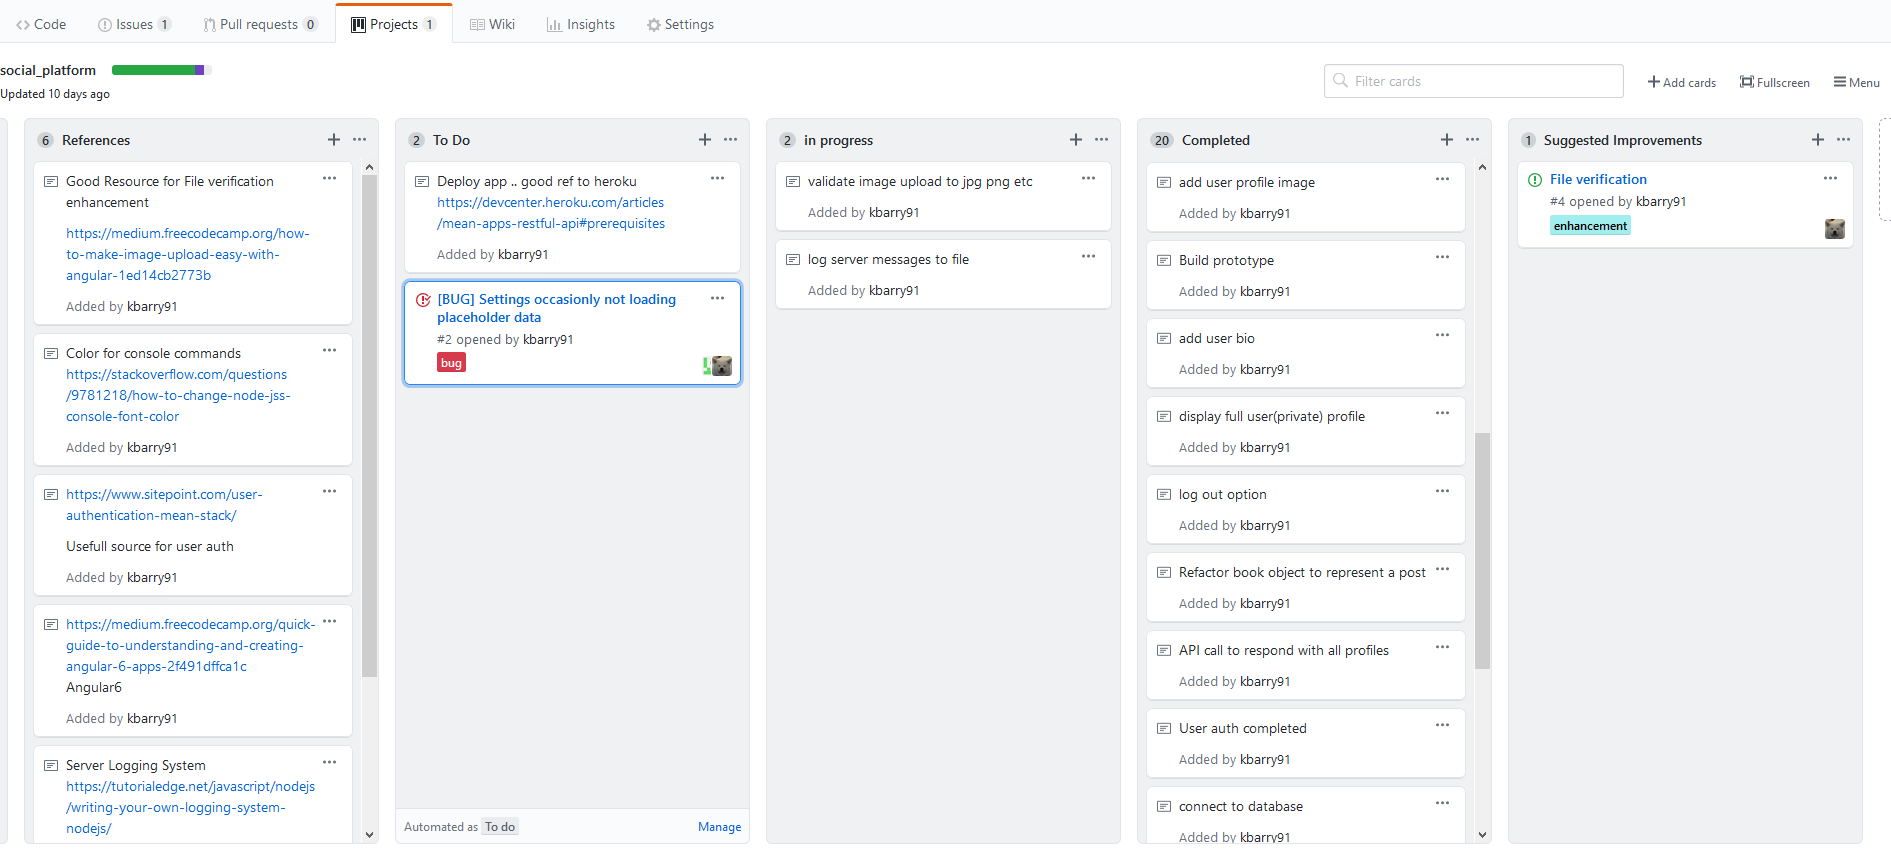
\includegraphics[width=\linewidth]{img/kanban.PNG}
  \caption{Github Kanban}
  \label{fig:kanban}
\end{figure}

Figure  ~\ref{fig:kanban} above contains a snapshot of the projects Kanban board during development using the online project utility available on Github. This allowed us, as a team, to see at any point in time, what tasks needing doing, which were in progress or completed, while also tracking bugs and and a section to propose improvements.

% ========================== Sprints   ========================== 
\subsection{Sprints}
The term Sprint is mainly used in the Scrum framework of the Agile methodology and for our project worked hand-in-hand with Kanban. A Sprint is a timed iteration of the continuous development cycle with a scrum being a meeting style discussion used to adapt feedback. During development our default sprint duration was one week starting directly after each weekly review with our supervisor and ending at the following review where we would conduct a sprint plan. The aim of the sprint plan is to as a team reach two key decisions, \textbf{Sprint goal} what can be achieved in the sprint and \textbf{Sprint Backlog} the tasks to be completed in order to achieve the goal. During each sprint plan we would we would analyze the Kanban and discuss the following topics:

\begin{enumerate}
  \item What did we complete in our preceding sprint?
  \item What issues did we face?
  \item Is anything preventing us from progressing with a feature?
  \item Do any features need improvement?
  \item What backlog items to be implemented in the next sprint?
  \item What backlog items can we implement in the next sprint?
\end{enumerate}

% ========================== Choice of tech  ========================== 
\section{Selection Criteria}
During the initial planning phases of the project, we evaluated numerous varying frameworks and technology stacks. From Java based Spring framework to Python's flask. As a team sat down to decide on the choice of technology and frameworks we would use. To do this we evaluated our project as a whole and began designing a criteria that we would base our final decision on. 

The criteria for selecting an architecture was based on :
\begin{enumerate}
  \item The type of web application we are trying to build.
  \item Implementation of 3 tier architecture.
  \item Server side must be easy to write and maintainable.
  \item Languages that need to be improved or learned to use framework.
  \item Use of database alongside server.
\end{enumerate}
Overall, based on the above criteria, we decided th         at the best solution for our project was to use the \textbf{MEAN} stack framework supported by Angular CLI. The Mean Stack provides multiple benefits which simplify the development of single page web applications with a 3-tier architecture. 

\begin{figure}[H]
  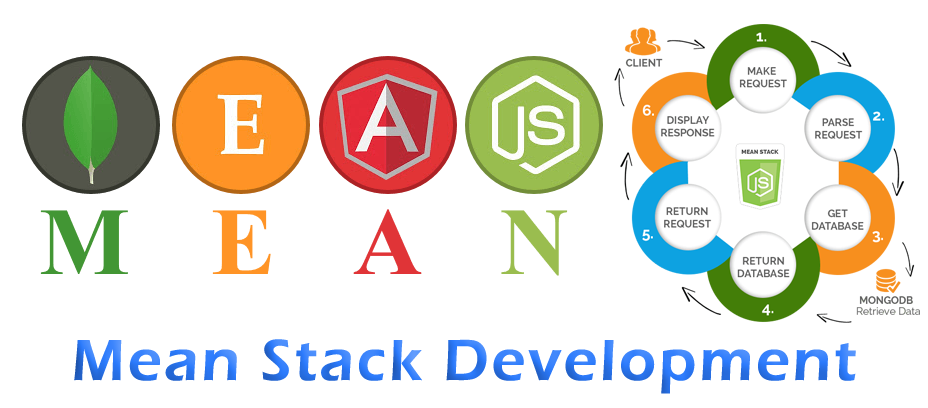
\includegraphics[width=\linewidth]{img/msd.png}
  \caption{Mean Stack Development}
  \label{fig:mena-stack}
\end{figure}

A major benefit of the MEAN stack is that it would enable us to develop everything from the Angular client ,to the Node server API all using JavaScript libraries. This allowing us to gain vast knowledge and increase our skill set in all areas of full-stack JavaScript applications. Another benefit of using MEAN stack is the increasing number of JavaScript libraries and Node modules available to aid development such as \textit{Mongoose} for adapting \textit{MongoDB} and \textit{Passport.Js} for server side authentication. In Section \ref{meanstack} we delve into more detail, giving a much broader explanation of the MEAN stack and the features that made it the go-to choice for Techbook.


% ========================== Testing , pass fail metrics  ========================== 
\section{Testing , Success and Failure Metrics} 
As defined briefly in Section \ref{metrics} \texttt{Metrics for success or failure} our conditions were mainly focused and evaluated by user interaction. With the intention of monitoring  success we decided on tests to evaluate each metric:

\begin{enumerate}
  \item \textbf{\textit{A  concise,  yet  comprehensive  dissertation  which  can  be  understood  by
anyone  regardless  of  their  initial  knowledge  of  the  technologies  implemented.}} To be able to test the simplicity and understanding gathered from the reader of the dissertation we decided to review ten people. We decided to choose five people each of different technological knowledge to review sections of the dissertation. We split the groups into technical and not technical minded people getting the technical group to review Chapters \textit{4, 5 and 6} whilst the non technical group would read Chapters \textit{1, 3 and 7}. Following this asking each tester to summarize briefly in around 5 sentences their findings and assess their understanding of the project on a scale of 1-10. We could then make adjustments based on the feedback received and repeat this step.

  \item \textbf{\textit{ Simple, easy to use, functional web application}}. As testing this ourselves we felt it would have too much bias as we would know how the system worked so we felt outsourcing testers again was the best solution. To test this we would host prototyped versions of the build throughout the development process. Only provided the testers with a link and no previous explanation on how the site worked. Subsequently we would again have the testers report back to us with a rating based on the usability of the site from 1-10 and any pros cons they noted while using the application.
  
  \item \textbf{\textit{A social platform that actually develops an online community}}. We have to be able to evaluate if the site actually functions as a social media platform .To confirm with the \textit{Data Protection Act 2018} \cite{dpa} we decided it would be best not to monitor users direct activity. Although it is hard to decide a concrete fixed value for what would be a success as the amount of users subscribed to the service would be growing, the best way to test this is logging when users follow another profile and when they post or comment on articles. Integrating a server logging system into the project that does not store confidential information would give us a rough idea of the result.
  
  \item \textbf{\textit{Teamwork Collaboration}}. We felt from a project management perspective and by researching the importance of a good team in industry, that we would measure the success of the team. In general teamwork effort is something not easily measured in a definitive way. With each weekly team meeting we would take time to reflect on how we resolved issues and while looking at the strengths and weaknesses of our collaborative efforts. 

\end{enumerate}
 The graphs in Figure \ref{tikz:graphs} briefly illustrate the iterative process taken for the purpose of pushing the above metrics to a success.
 
\begin{figure}[H]
  \centering
  \begin{tikzpicture}[node distance=1cm and 6cm]
    \node (a) [rect] {1. Gather requirements for feature};
    \node (b) [oval,right= of a] {2. Implement feature};
    \node (c) [rect, below= of b] {3. User testing};
    \node (d) [oval,below= of a] {4. Review & evaluate feedback};
  \draw [line] (a) -- (b) -- (c) -- (d) -- (a) ;
  \end{tikzpicture}
  \caption{Success / Failure Test cycle}
  \label{tikz:graphs}
\end{figure}







